\chapter{Esercizio 10}

\subsection{Testo}

\begin{center}
    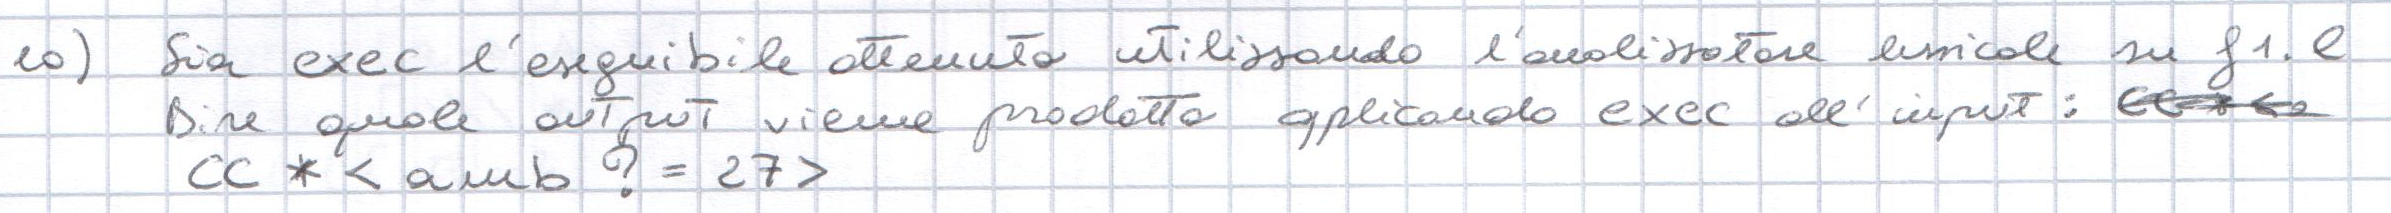
\includegraphics[scale=0.2]{Chapters/Img/10text.png}\\
\end{center} 

\subsection{Soluzione}
f1.l
\begin{lstlisting}
    %{
    
    %}

    digit [0-9]
    letters [a-z,A-Z]
    other [\\\*\?"<"]
    id ({other}|{digit}|{letters})+

    %%
    ({other})?({other})?({id})({digit})+({id})?   {printf("SI ");}
    {id}   {printf("FORSE ");}
    .   {printf("NO ");}

    %%
    int yywrap() {
    return 1;
    }

    int main() {
    yylex();
    }
\end{lstlisting}

\subsection{Risposta}
\begin{lstlisting}
    Input: CC*<amb?=27> 
    Output: FORSE NO SI NO
\end{lstlisting}

Notare che (a | b)+ matcha con ab, abbaaab, ...